\chapter*{Acronyms}
    \begin{acronym}
        \acro{ccm}[CCM]{Centre for Cold Matter}
        \acro{rb87}[\(^{87}\)Rb]{Rubidium-87}
        \acro{rb85}[\(^{85}\)Rb]{Rubidium-85}
        \acro{mot}[MOT]{Magneto-optical Trap}
        \acro{aom}[AOM]{Acousto-optic Modulator}
        \acro{eom}[EOM]{Electro-optic Modulator}
        \acro{pm}[PM]{Polarisation-Maintaining}
        \acro{qwp}[QWP]{Quarter-wave Plate}
        \acro{hwp}[HWP]{Half-wave Plate}
        \acro{mfd}[MFD]{Mode Field Diameter}
        \acro{ppln}[PPLN]{Periodically Poled Lithium Niobate}
        \acro{pll}[PLL]{Phase-Locked Loop}
        \acro{fpga}[FPGA]{Field-Programmable Gate Array}
        \acro{edfa}[EDFA]{Erbium-Doped Fibre Amplifier}
        \acro{ecdl}[ECDL]{External-Cavity Diode Laser}
        \acro{ttl}[TTL]{Transistor-transistor Logic Circuit}
        \acro{ni}[NI]{National Instruments}
        \acro{daq}[DAQ]{Data Acquisition}
        \acro{vco}[VCO]{Voltage-Controlled Oscillator}
        \acro{adc}[ADC]{Analogue-to-Digital Converter}
        \acro{dac}[DAC]{Digital-to-Analogue Converter}
        \acro{hal}[HAL]{Hardware Abstraction Layer}
        \acro{spi}[SPI]{Serial Programming Interface}
        \acro{dds}[DDS]{Direct Digital Synthesiser}
        \acrodefplural{aom}[AOMs]{Acousto-optic Modulators}
        \acrodefplural{ecdl}[ECDLs]{External-Cavity Diode Lasers}
        \acrodefplural{edfa}[EDFAs]{Erbium-Doped Fibre Amplifiers}
        \acrodefplural{ttl}[TTLs]{Transistor-transistor Logic Circuits}
        \acrodefplural{mots}[MOTs]{Magneto-optical Traps}
        \acro{pbs}[PBS]{Polarising beam-splitter}
        \acro{dro}[DRO]{Dielectric Resonator Oscillator}
    \end{acronym}


\chapter{Laser Systems}
\label{chap:setup}
This chapter provides a description of the hardware that makes up the experiment. Over the course of the project, the complexity of the experiment necessarily increased. The setup is presented in a bottom-up approach, starting from the most fundamental components, to provide a clear overview of the system. \\

\verysubsection{To-Do}
\begin{itemize}\item Figures describing each of the lasers
    \item Describe 3D and 2D MOT setups  
    \item Imaging systems
    \item Microwave synthesisers
    \item Raman Assembly
    \item MOT light distribution
\end{itemize}
\section{Chapter Overview}\label{sec:setup_overview}
The first two sections describe the two commercial laser systems used in this experiment. The \Muquans laser system which generates the light used for cooling and repump in the 2D and 3D \acp{mots}, referred to as the \acs{mot} light. The design and operation of this laser is given in \SectionRef{sec:setup_muquans}. A secondary laser system, built by MSquared, is used to generate light to drive Raman transitions between two hyperfine ground states in \ac{rb87}\footnote{The \Muquans laser also has a pair of lasers designed for driving Raman transitions, but these are not used in this experiment. \SectionRef{sec:setup_msquared} gives an explanation for this.}, otherwise referred to as Raman light. This is described in \SectionRef{sec:setup_msquared}.This is followed by a description of the vacuum chamber in \SectionRef{sec:setup_chamber} which contains both the 2D \ac{mot} (\SectionRef{subsec:setup_2DMOT}) and the 3D \ac{mot} (\SectionRef{subsec:setup_3DMOT}).  

\section{The \Muquans Laser System}\label{sec:setup_muquans}
\verysubsection{To-Do}
\begin{itemize}
    \item Laser Schematic
    \item Plots of lock signals
    \item DDS Serial communication
    \item Power output, stability
    \item Ref for error signal generation by current modulation
    \item Move some of this to appendix
\end{itemize}
All the \ac{mot} light in this experiment was generated by the \Muquans laser \cite{muquansWebPage}. \Muquans is a French laser company that is a spin-off from the Institut d'Optique and Observatoire de Paris. Consequently, their technology has been developed over a long history of performing experiments into atom interferometry using Rubidium. A schematic of this laser system is shown in \FigureRef{fig:muquans_schematic}. The \Muquans laser is comprised of four 1560nm \acp{ecdls} which are frequency-doubled to produce light at wavelengths close to 780nm. The telecommunications industry, which relies heavily on light in the 1530-1565nm wavelength band for optical communications, has motivated a rapid development in low-noise, robust lasers. In particular, this has enabled a design which does not require free-space optics and is much more resilient to effects such as temperature changes and vibrations, when compared to more conventional 780nm laser systems. The \Muquans laser contains one master laser \footnote{see \SectionRef{subsec:muquans_master} for more details}, which is locked to the \(F = 3 \rightarrow F' = 3,4\) crossover point in \ac{rb85}, and serves as an absolute frequency reference. The other three slave lasers are used for output. The first one is used to provide lightAll the \ac{mot} light in this experiment was generated by the \Muquans laser \cite{muquansWebPage}. \Muquans is a French laser company that is a spin-off from the Institut d'Optique and Observatoire de Paris. Consequently, their technology has been developed over a long history of performing experiments into atom interferometry using Rubidium. A schematic of this laser system is shown in \FigureRef{fig:muquans_schematic}. The \Muquans laser is comprised of four 1560nm \acp{ECDLs} which are frequency-doubled to produce light at wavelengths close to 780nm. The telecommunications industry, which relies heavily on light in the 1530-1565nm wavelength band for optical communications, has motivated a rapid development in low-noise, robust lasers. In particular, this has enabled a design which does not require free-space optics and is much more resilient to effects such as temperature changes and vibrations, when compared to more conventional 780nm laser systems. The \Muquans laser contains one master laser \footnote{see \SectionRef{subsec:muquans_master} for more details}, which is locked to the \(F = 3 \rightarrow F' = 3,4\) crossover point in \ac{rb85}, and serves as an absolute frequency reference. The other three slave lasers are used for output. The first one is used to provide light for cooling, as well as repump light by modulating the phase of this laser using an \ac{eom}. The other two make up a pair of lasers for driving Raman transitions. One laser is frequency-offset locked to the master and the other is phase-locked to the first, to ensure that the relative phase between the two lasers is constant. It should be noted that this Raman laser was not used in this experiment, so will not be discussed in great detail. Each of these slave lasers is amplified in an \ac{edfa} before being frequency doubled in a \ac{ppln} and passed through an \ac{aom} which is used to control the output power during the experiment.  for cooling, as well as repump light by modulating the phase of this laser using an \ac{eom}. The other two make up a pair of lasers for driving Raman transitions. One laser is frequency-offset locked to the master and the other is phase-locked to the first, to ensure that the relative phase between the two lasers is constant. It should be noted that this Raman laser was not used in this experiment, so will not be discussed in great detail. Each of these slave lasers is amplified in an \ac{edfa} before being frequency doubled in a \ac{ppln} and passed through an \ac{aom} which is used to control the output power during the experiment. 
\begin{figure}
    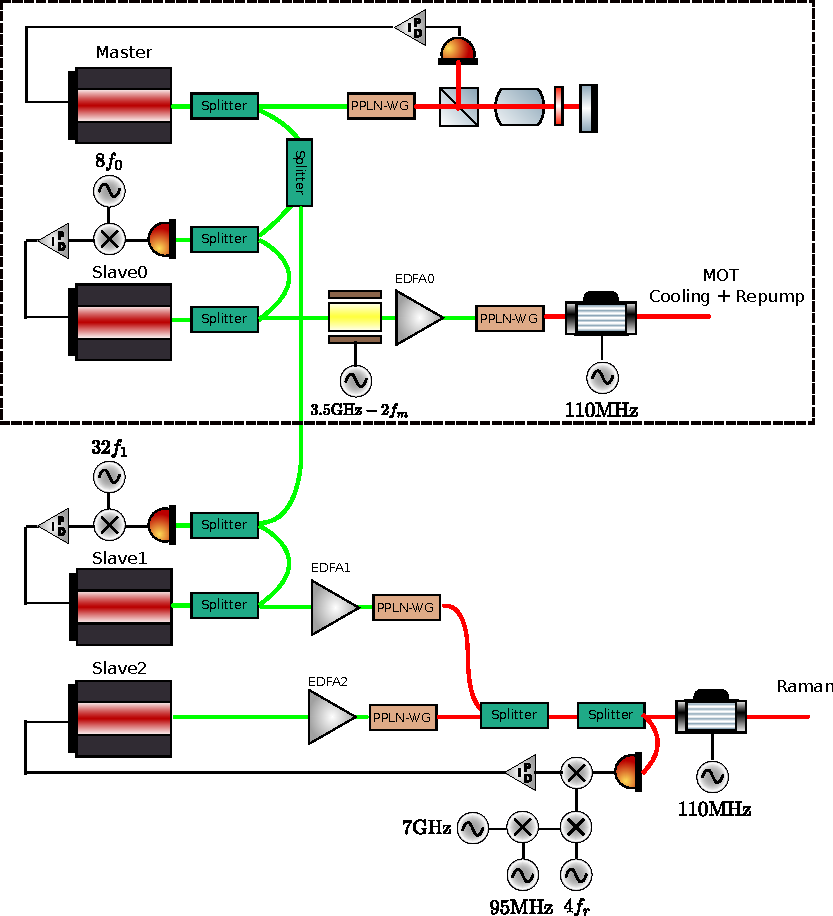
\includegraphics{muquans_schematic}
    \caption[\Muquans Laser System Diagram]{Schematic of the \Muquans laser system. Each output laser is derived from a 1560nm \acs{ecdl} (shown in green) which is amplified using an \acs{edfa} and then frequency-doubled to 780nm using a \acs{ppln} crystal. A master laser is locked to the 3,4 crossover in \ac{rb85} and the output lasers are offset-locked to their corresponding frequencies. The dashed region indicates the components used for generating light for the \acp{mots}, which was the only function of this laser for this experiment.}\label{fig:muquans_schematic}
\end{figure}
\subsection{Absolute Frequency Reference} \label{subsec:muquans_master}
The purpose of the master laser is to provide an absolute frequency reference so that the frequency of the output lasers can be controlled by comparing the difference frequency between them and the master. Lasers with linewidths narrower than their natural linewidth can be achieved by using a servo to stabilise their frequency and is essential for any experiment that requires laser light of a precise frequency. The frequency reference for the master is obtained using saturated absorption spectroscopy inside a Rubidium vapor cell. The sub-Doppler features in this spectrum are insensitive to temperature changes, and under sufficiently weak laser power have linewidths close to the natural linewidth of Rubidium (\(\Gamma \sim 2\pi \times 6\)MHz). \FigureRef{fig:muquans_satspec} shows the saturated absorption spectrum using the \Muquans master laser. This is obtained by fine adjustment of the temperature of the master \ac{ecdl}. The laser is set to lock to the crossover resonance between the \(F = 3 \rightarrow F' = 3\) and \(F = 3 \rightarrow F' =4 \) transitions in \ac{rb85} (indicated as \(b)\)), which is the strongest feature in the spectrum as well as being relatively close the the cooling transition in \ac{rb87} (indicated as \(a)\)).   
\begin{figure}
    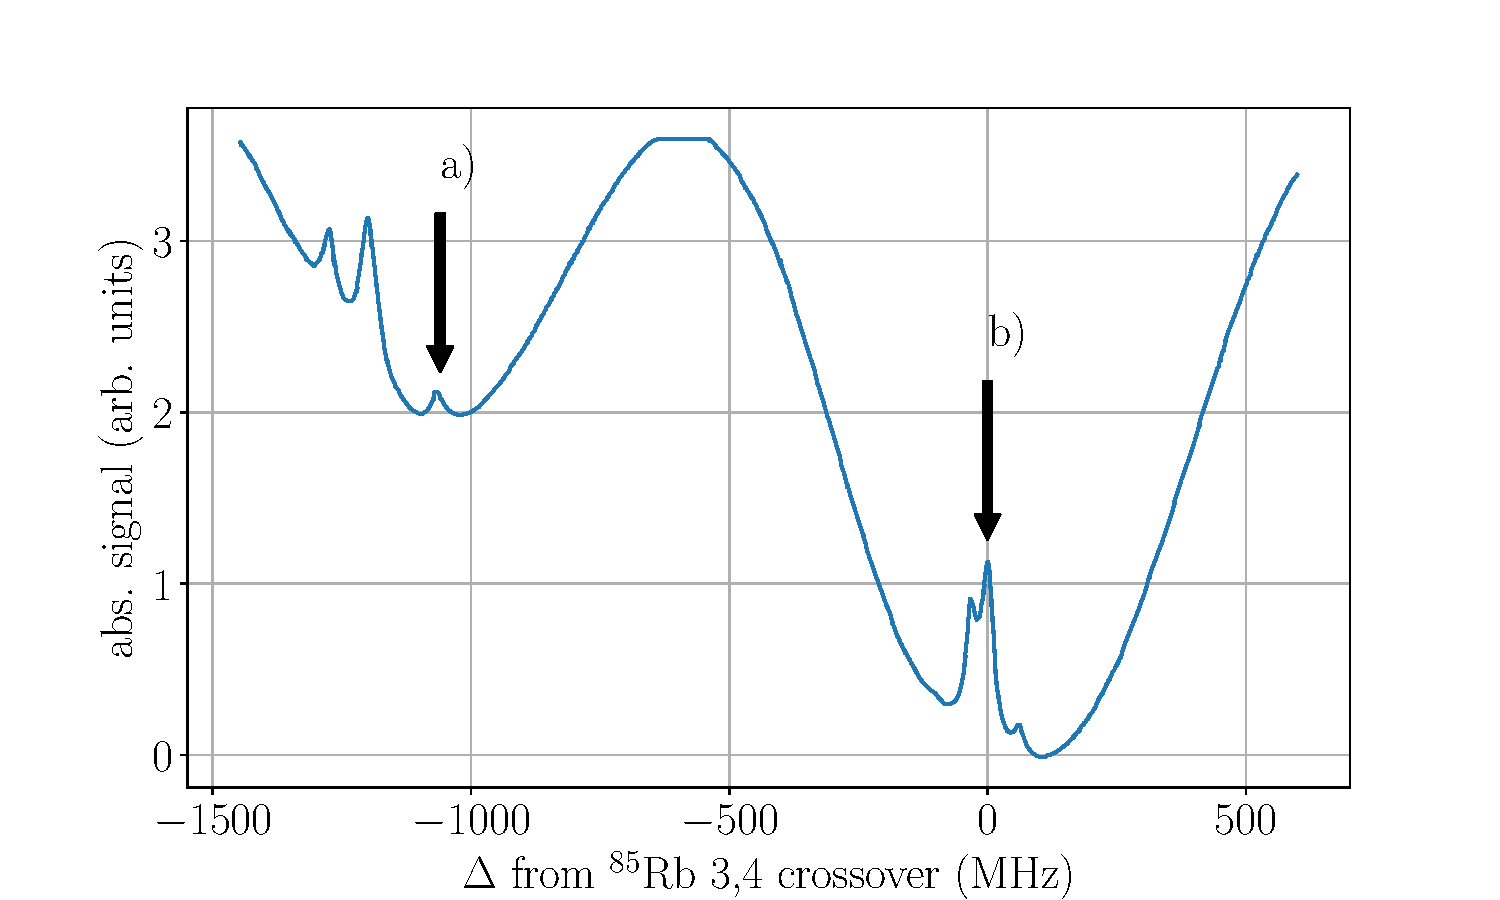
\includegraphics[width=0.6\textwidth]{sat_spec}
    \caption[Saturated absorption spectroscopy of the \Muquans master laser.]{Saturated absorption spectroscopy using the Rubidium vapour cell in the \Muquans laser. The absorption features indicated are \(a)\): the \(F = 2 \rightarrow F' = 3\) transition in \ac{rb87} and \(b)\): the crossover resonance between the \(F = 3 \rightarrow F' = 3\) and \(F = 3 \rightarrow F' =4 \) transitions in \ac{rb85} which is used to lock the frequency of the master laser.}
    \label{fig:muquans_satspec}
\end{figure}
\begin{figure}
    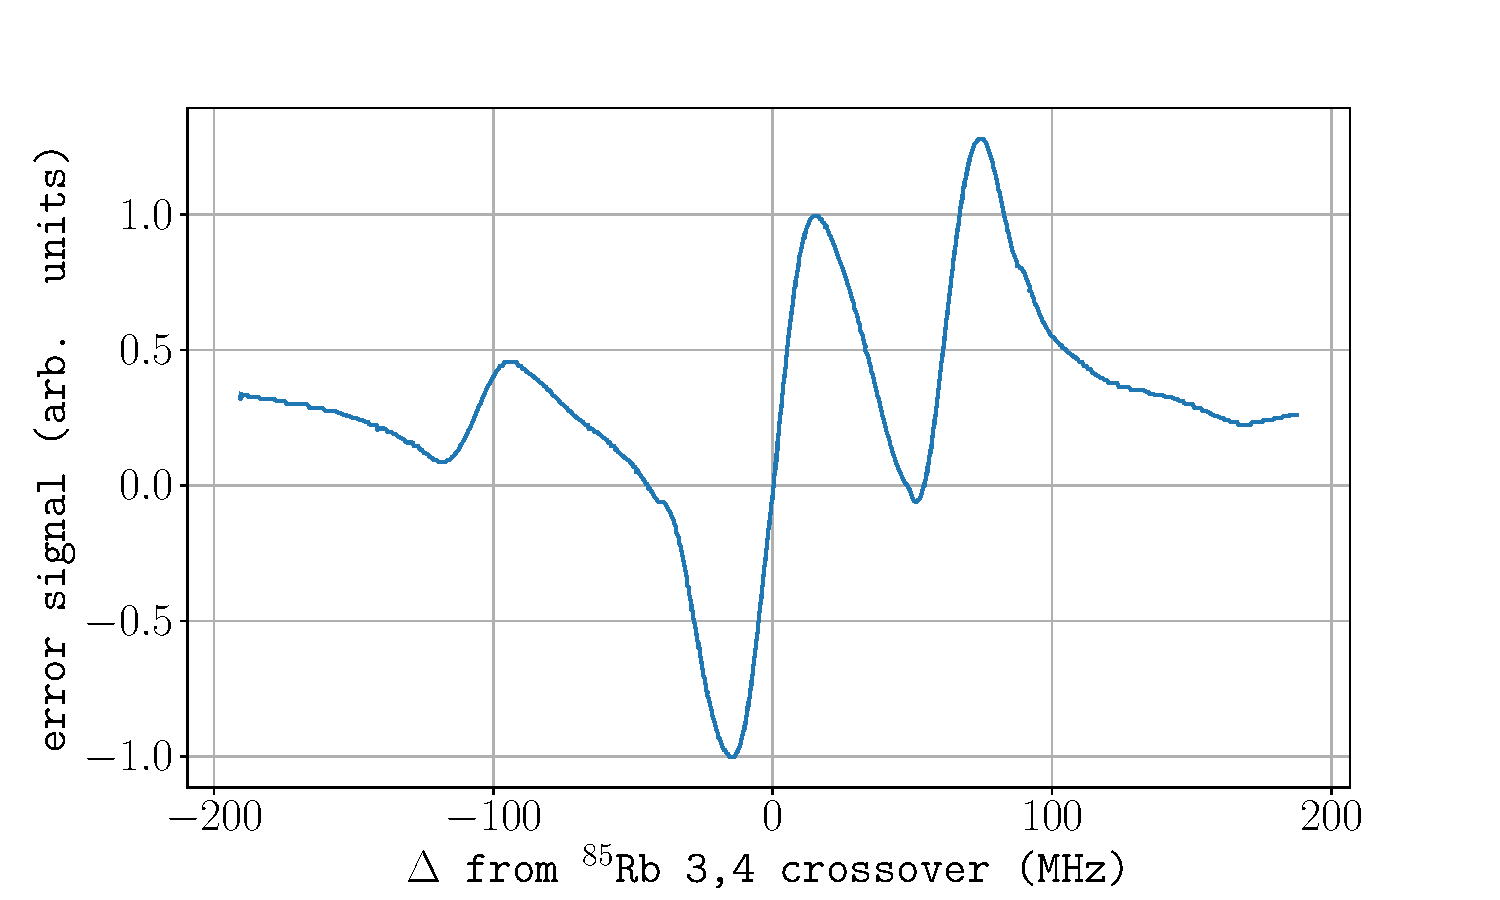
\includegraphics[width=0.6\textwidth]{error_signal}
    \caption[Error Signal for the \Muquans master servo.]{Error signal obtained by modulating the laser current. Close to the lock point, the signal is approximately linear. This signal is used in a feed-back loop to correct for frequency changes of the master laser.}
    \label{fig:muquans:error_signal}
\end{figure}
Some form of feed-back onto the master laser is required to keep its frequency fixed. The simplest way to achieve this is to use a signal that is linearly proportional to the deviation in frequency from the set-point, if one exists. The frequency of the laser is modulated by weakly modulating the current to the master \ac{ecdl}. {\textbf add more detail about the error signal lineshape} The error signal shown in \FigureRef{fig:muquans_errorsignal} is obtained by demodulating the absorption signal using a lock-in amplifier. In fact, this current modulation is always present on the master laser and the saturated absorption spectrum shown previously has been processed to average out the effects from this fast frequency modulation. In addition to proportional feed-back from the error signal, the servo that controls the master frequency also contains an integrator to compensate for long-term drifts. Typically, these arise from external temperature changes and if unaccounted for, they could cause the laser to unlock. In the conditions of our laboratory, where the temperature is externally controlled, this has never occurred.  
\subsection{Generating MOT light}
\subsection{Raman light}
\subsection{Real-time Frequency Control}
\section{The M-Squared Laser System}\label{sec:setup_msquared}
\verysubsection{To-Do}
\begin{itemize}
    \item Schematic
    \item Raman PLL phase-noise
    \item Laser Control
    \item DCS module
\end{itemize}
\subsection{Laser Specifications}
\subsection{The DCS Control Module}
\subsection{Frequency Control of the Raman Lasers}
\subsection{Controlling the Phase Difference}
